\documentclass[oneside,a4paper,14pt]{extarticle}
\usepackage[a4paper,letterpaper,top=20mm,bottom=20mm,left=20mm,right=10mm]{geometry}
\usepackage[russian]{babel}
\usepackage{indentfirst}
\usepackage{graphicx}
\usepackage{caption}
\usepackage{titlesec}
\usepackage{minted, fancyvrb}

\titleformat{\section} {\normalsize\bfseries} {\thesection} {1em} {}
\titleformat{\subsection} {\normalsize\bfseries} {\thesubsection} {1em} {}
\titleformat{\subsubsection} {\normalsize\bfseries} {\thesubsection} {1em} {}
\renewcommand\baselinestretch{1.45}\normalsize
\setlength{\parindent}{1.25cm}

\begin{document}

\newpage
\thispagestyle{empty}
\begin{center}
	МИНИСТЕРСТВО НАУКИ И ВЫСШЕГО ОБРАЗОВАНИЯ РОССИЙСКОЙ ФЕДЕРАЦИИ ФЕДЕРАЛЬНОЕ ГОСУДАРСТВЕННОЕ БЮДЖЕТНОЕ ОБРАЗОВАТЕЛЬНОЕ УЧРЕЖДЕНИЕ ВЫСШЕГО ОБРАЗОВАНИЯ\\
	«ВЯТСКИЙ ГОСУДАРСТВЕННЫЙ УНИВЕРСИТЕТ»\\
	Институт математики и информационных систем\\
	Факультет автоматики и вычислительной техники\\
	Кафедра электронных вычислительных машин
\end{center}
\vspace{10mm}

\hfill
\begin{tabular}{l}
	\footnotesize Дата сдачи на проверку:                                          \\
	\footnotesize <<\rule[-1mm]{5mm}{0.10mm}\/>>\rule[-1mm]{20mm}{0.10mm}\ 2025 г. \\
	\footnotesize Проверено:                                                       \\
	\footnotesize <<\rule[-1mm]{5mm}{0.10mm}\/>>\rule[-1mm]{20mm}{0.10mm}\ 2025 г. \\
\end{tabular}
\vfill

\begin{center}
	ВНЕШНЯЯ СОРТИРОВКА ФАЙЛА. РАБОТА С ФОРМАМИ В LAZARUS.\\
	Отчёт по лабораторной работе №8\\
	по дисциплине\\
	<<Программирование>>\\
\end{center}
\vspace{25mm}
\noindent
\begin{tabular}{ll}
	Разработал студент гр. ИВТб-1301-05-00 & \rule[-1mm]{30mm}{0.10mm}\,/Черкасов А. А./   \\
	                                       & \hspace{8mm}\footnotesize(подпись)            \\
	Заведующая кафедры ЭВМ                 & \rule[-1mm]{30mm}{0.10mm}\,/Долженкова М. Л./ \\
	                                       & \hspace{8mm}\footnotesize(подпись)            \\
\end{tabular}

\noindent
\begin{tabular}{lp{58mm}r}
	Работа защищена &  & <<\rule[-1mm]{5mm}{0.10mm}\/>>\rule[-1mm]{30mm}{0.10mm}\ 2025 г.
\end{tabular}
\vfill

\begin{center}
	Киров\\
	2025
\end{center}

\newpage\thispagestyle{plain}

\section*{Цель}

Цель работы: Получение навыков реализации алгоритма внешней сортровки в Lazarus на языке pascal.

\section*{Задание}
\begin{itemize}
	\item[$-$] Написать программу с графическим интерфейсом для генерации и внешней сортировки файла.
  \item[$-$] Предусмотреть визуальное отображение работы программы с помощью инструментов Lazarus.
\end{itemize}

\section*{Решение}

Схемы алгоритмов решения задания представлены на рисунках 1.1, 1.2, 1.3, 1.4.1, 1.4.2, 1.5 и 1.6. Исходный код решений представлен в Приложениях А1.

\clearpage
\begin{figure}[H]
	\centering
	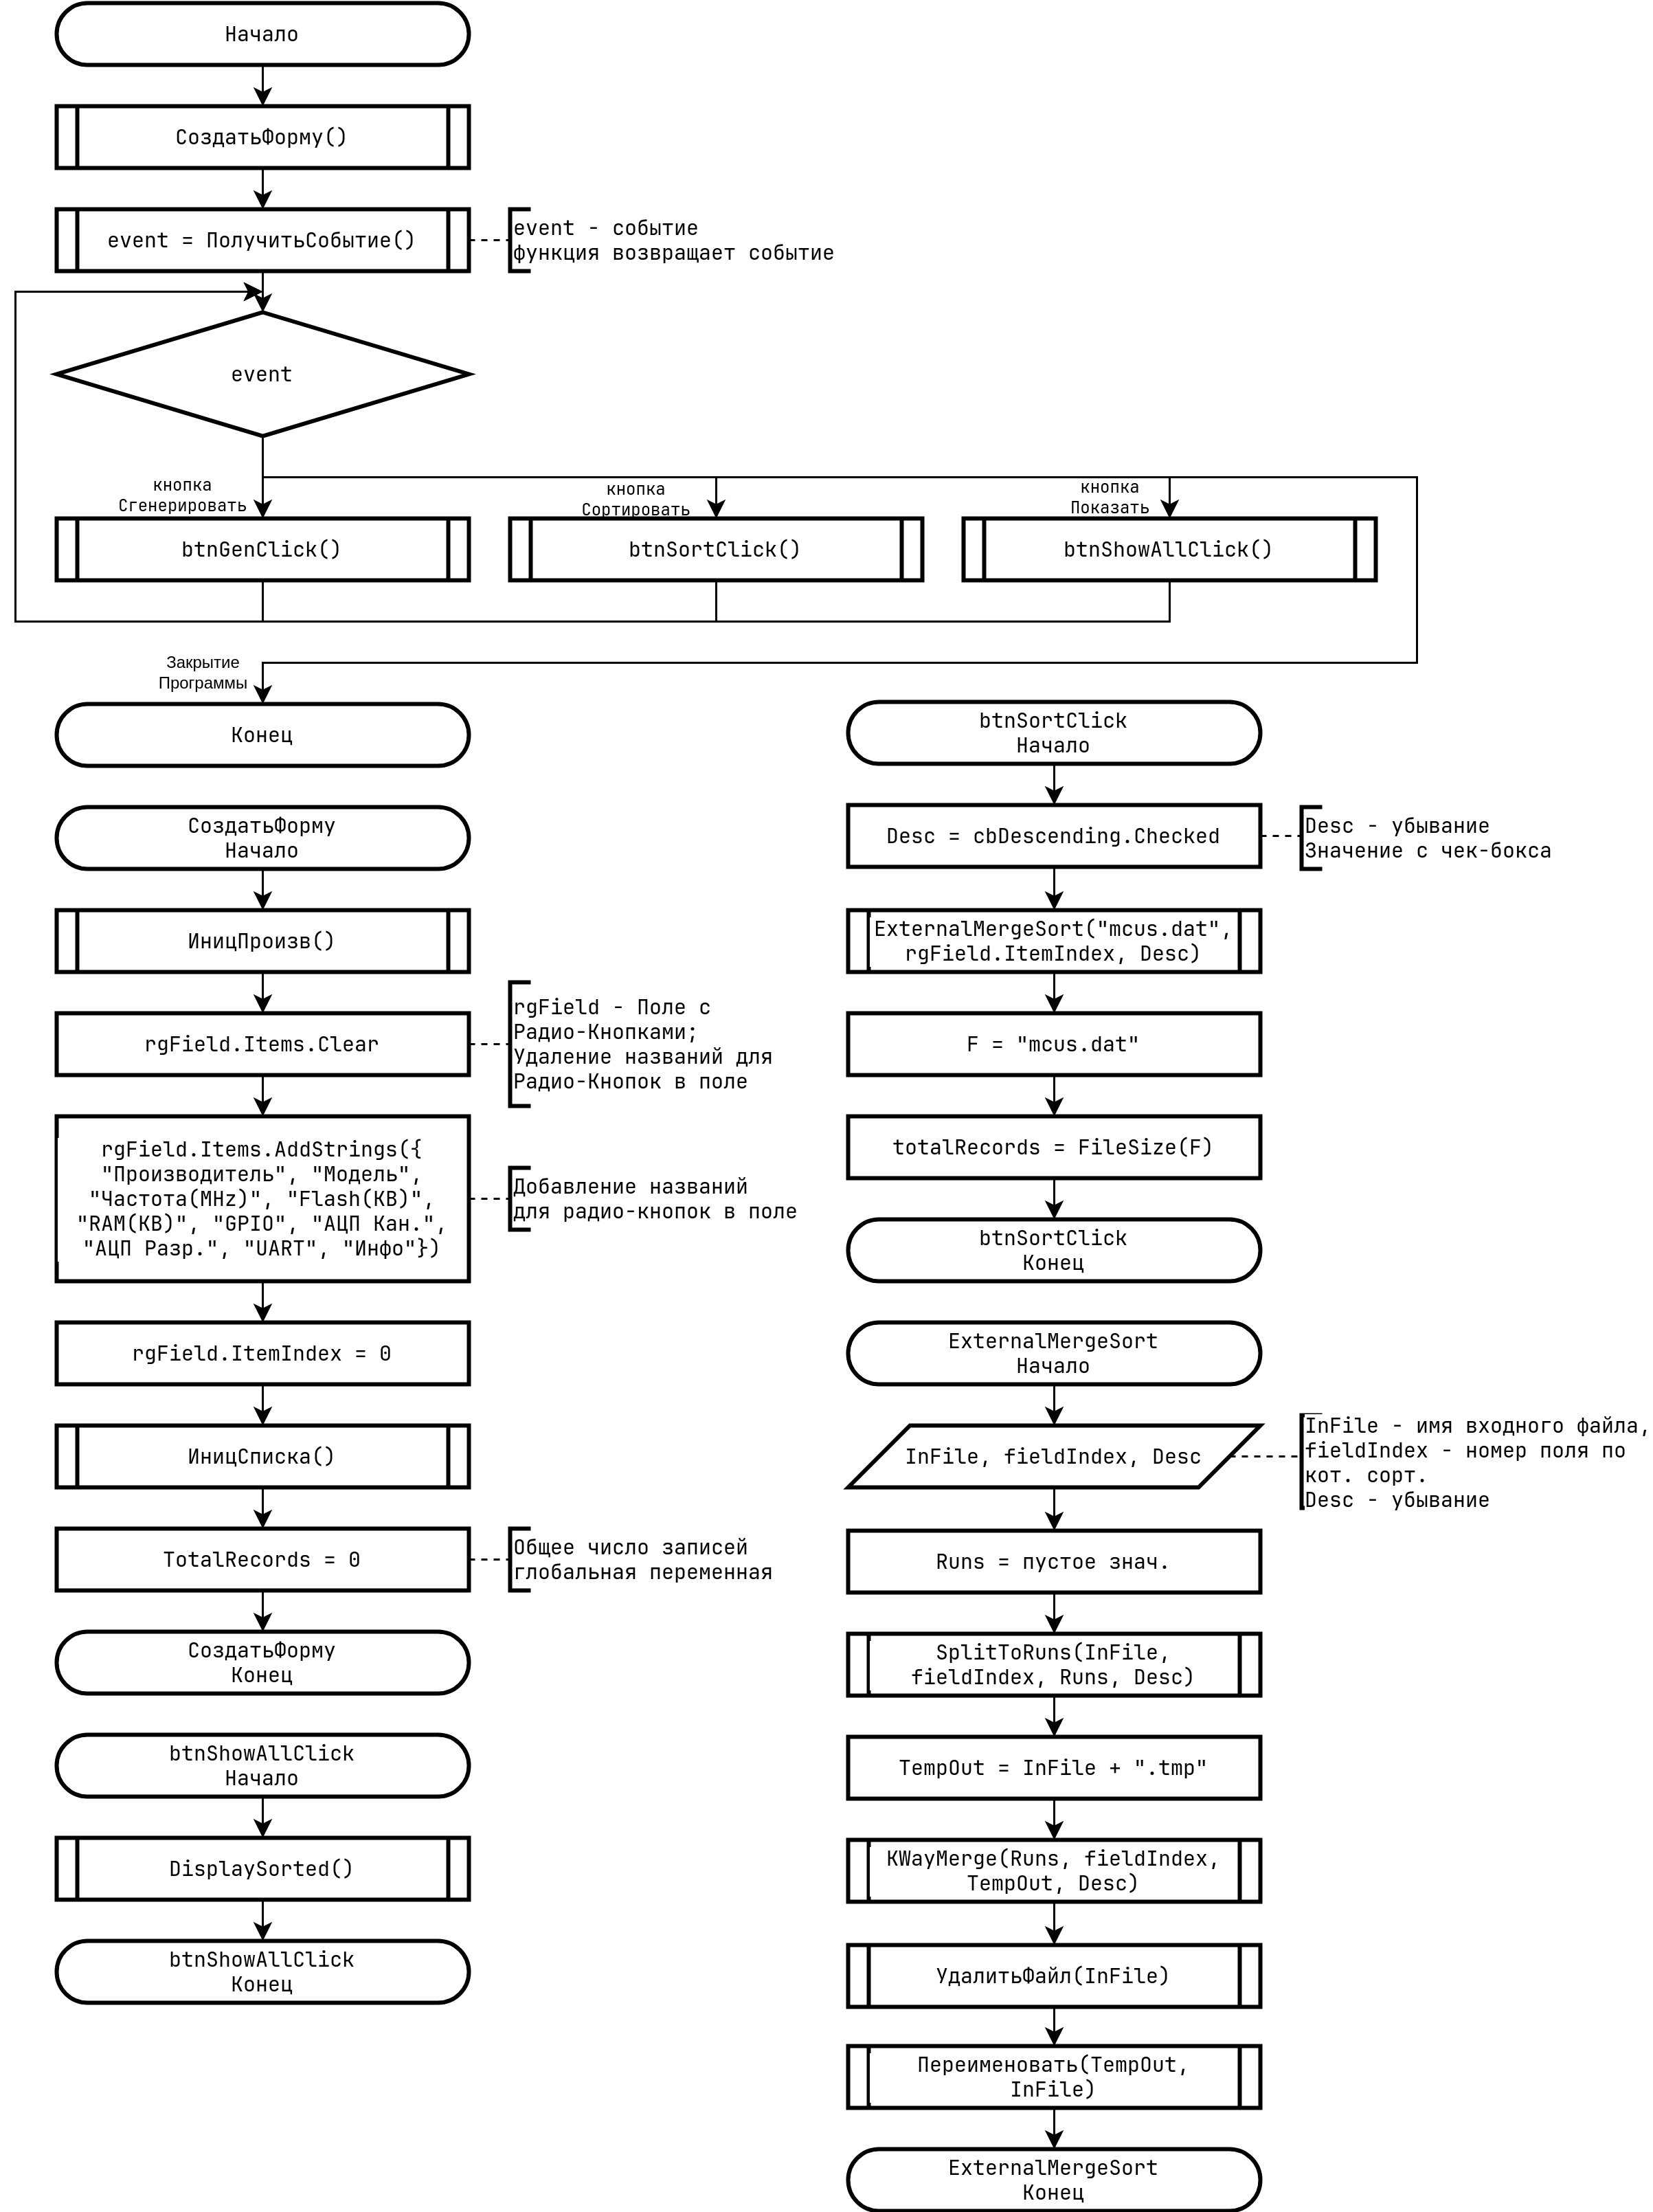
\includegraphics[height=0.85\textheight]{pics/flowchart1.png}
	\caption*{Рисунок 1.1 - Схемы алгоритмов главной программы, подпрограммы инициализации формы, подпрограмм нажатия на кнопки Показать и Сортировать, подпрограммы вызова внешней сортировки.}
\end{figure}

\clearpage
\begin{figure}[H]
	\centering
	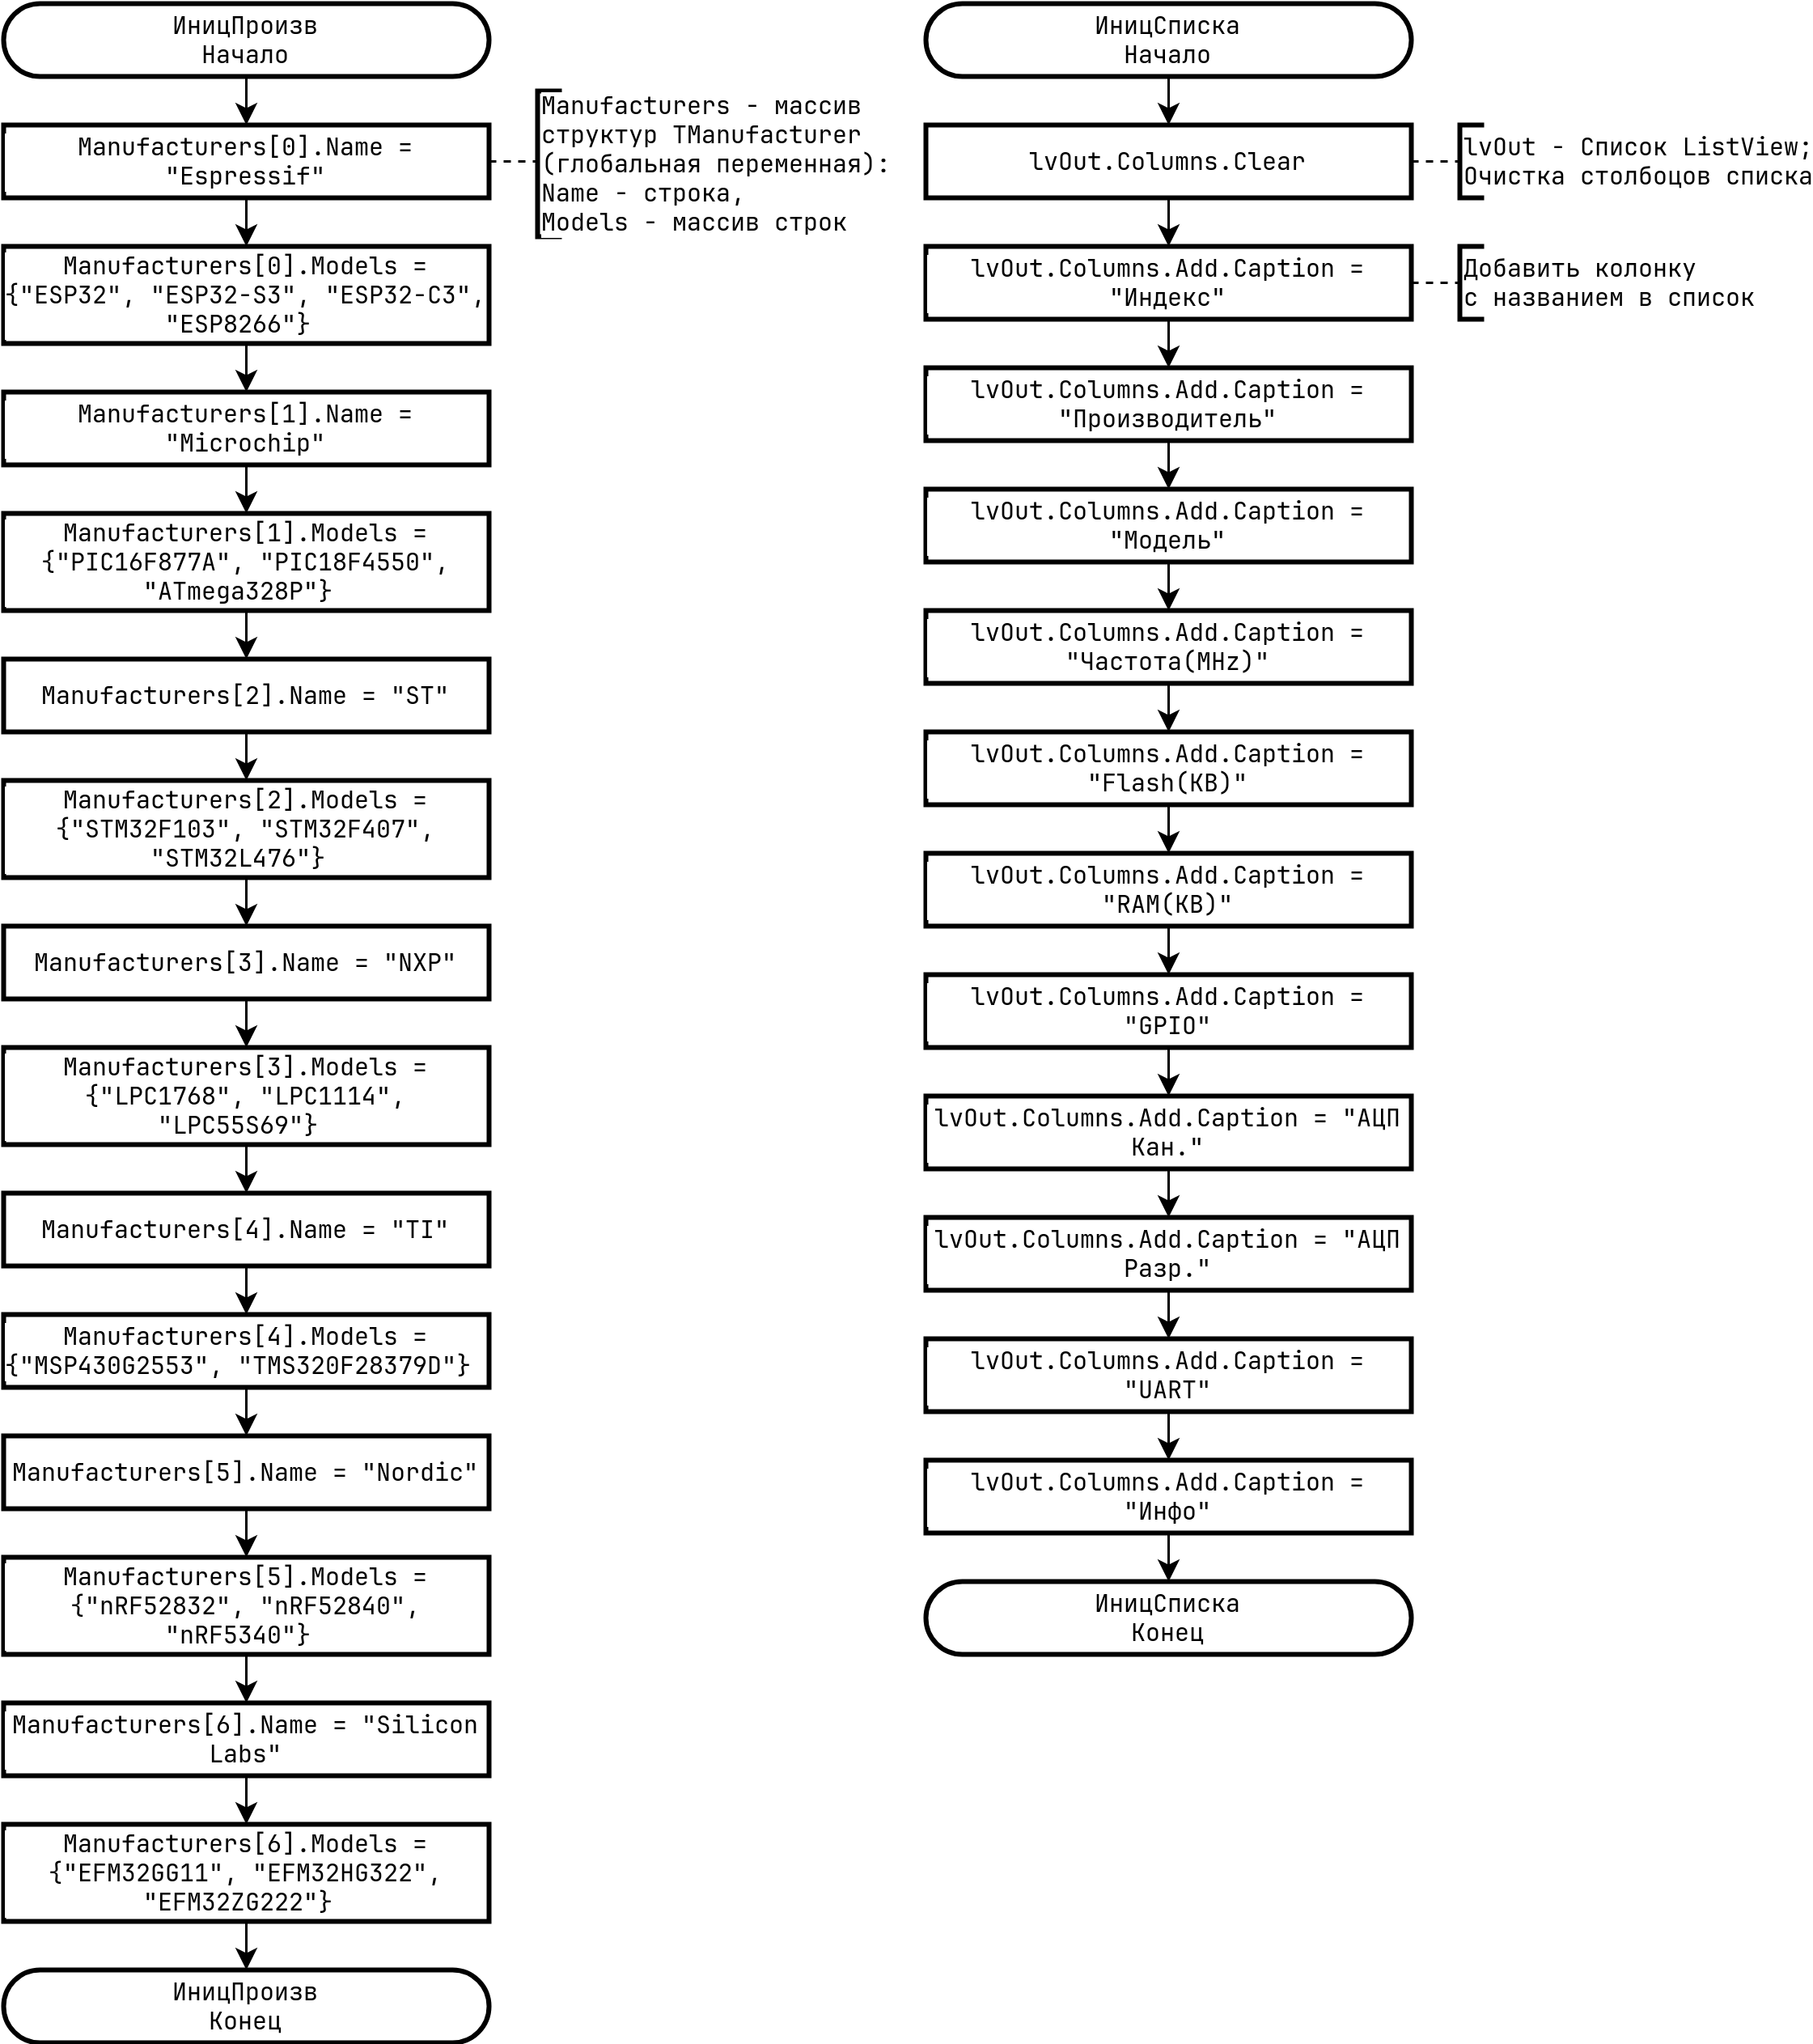
\includegraphics[width=0.95\textwidth]{pics/flowchart2.png}
	\caption*{Рисунок 1.2 - Схемы алгоритмов подпрограмм инициализации Производителей и Списка.}
\end{figure}

\clearpage
\begin{figure}[H]
	\centering
	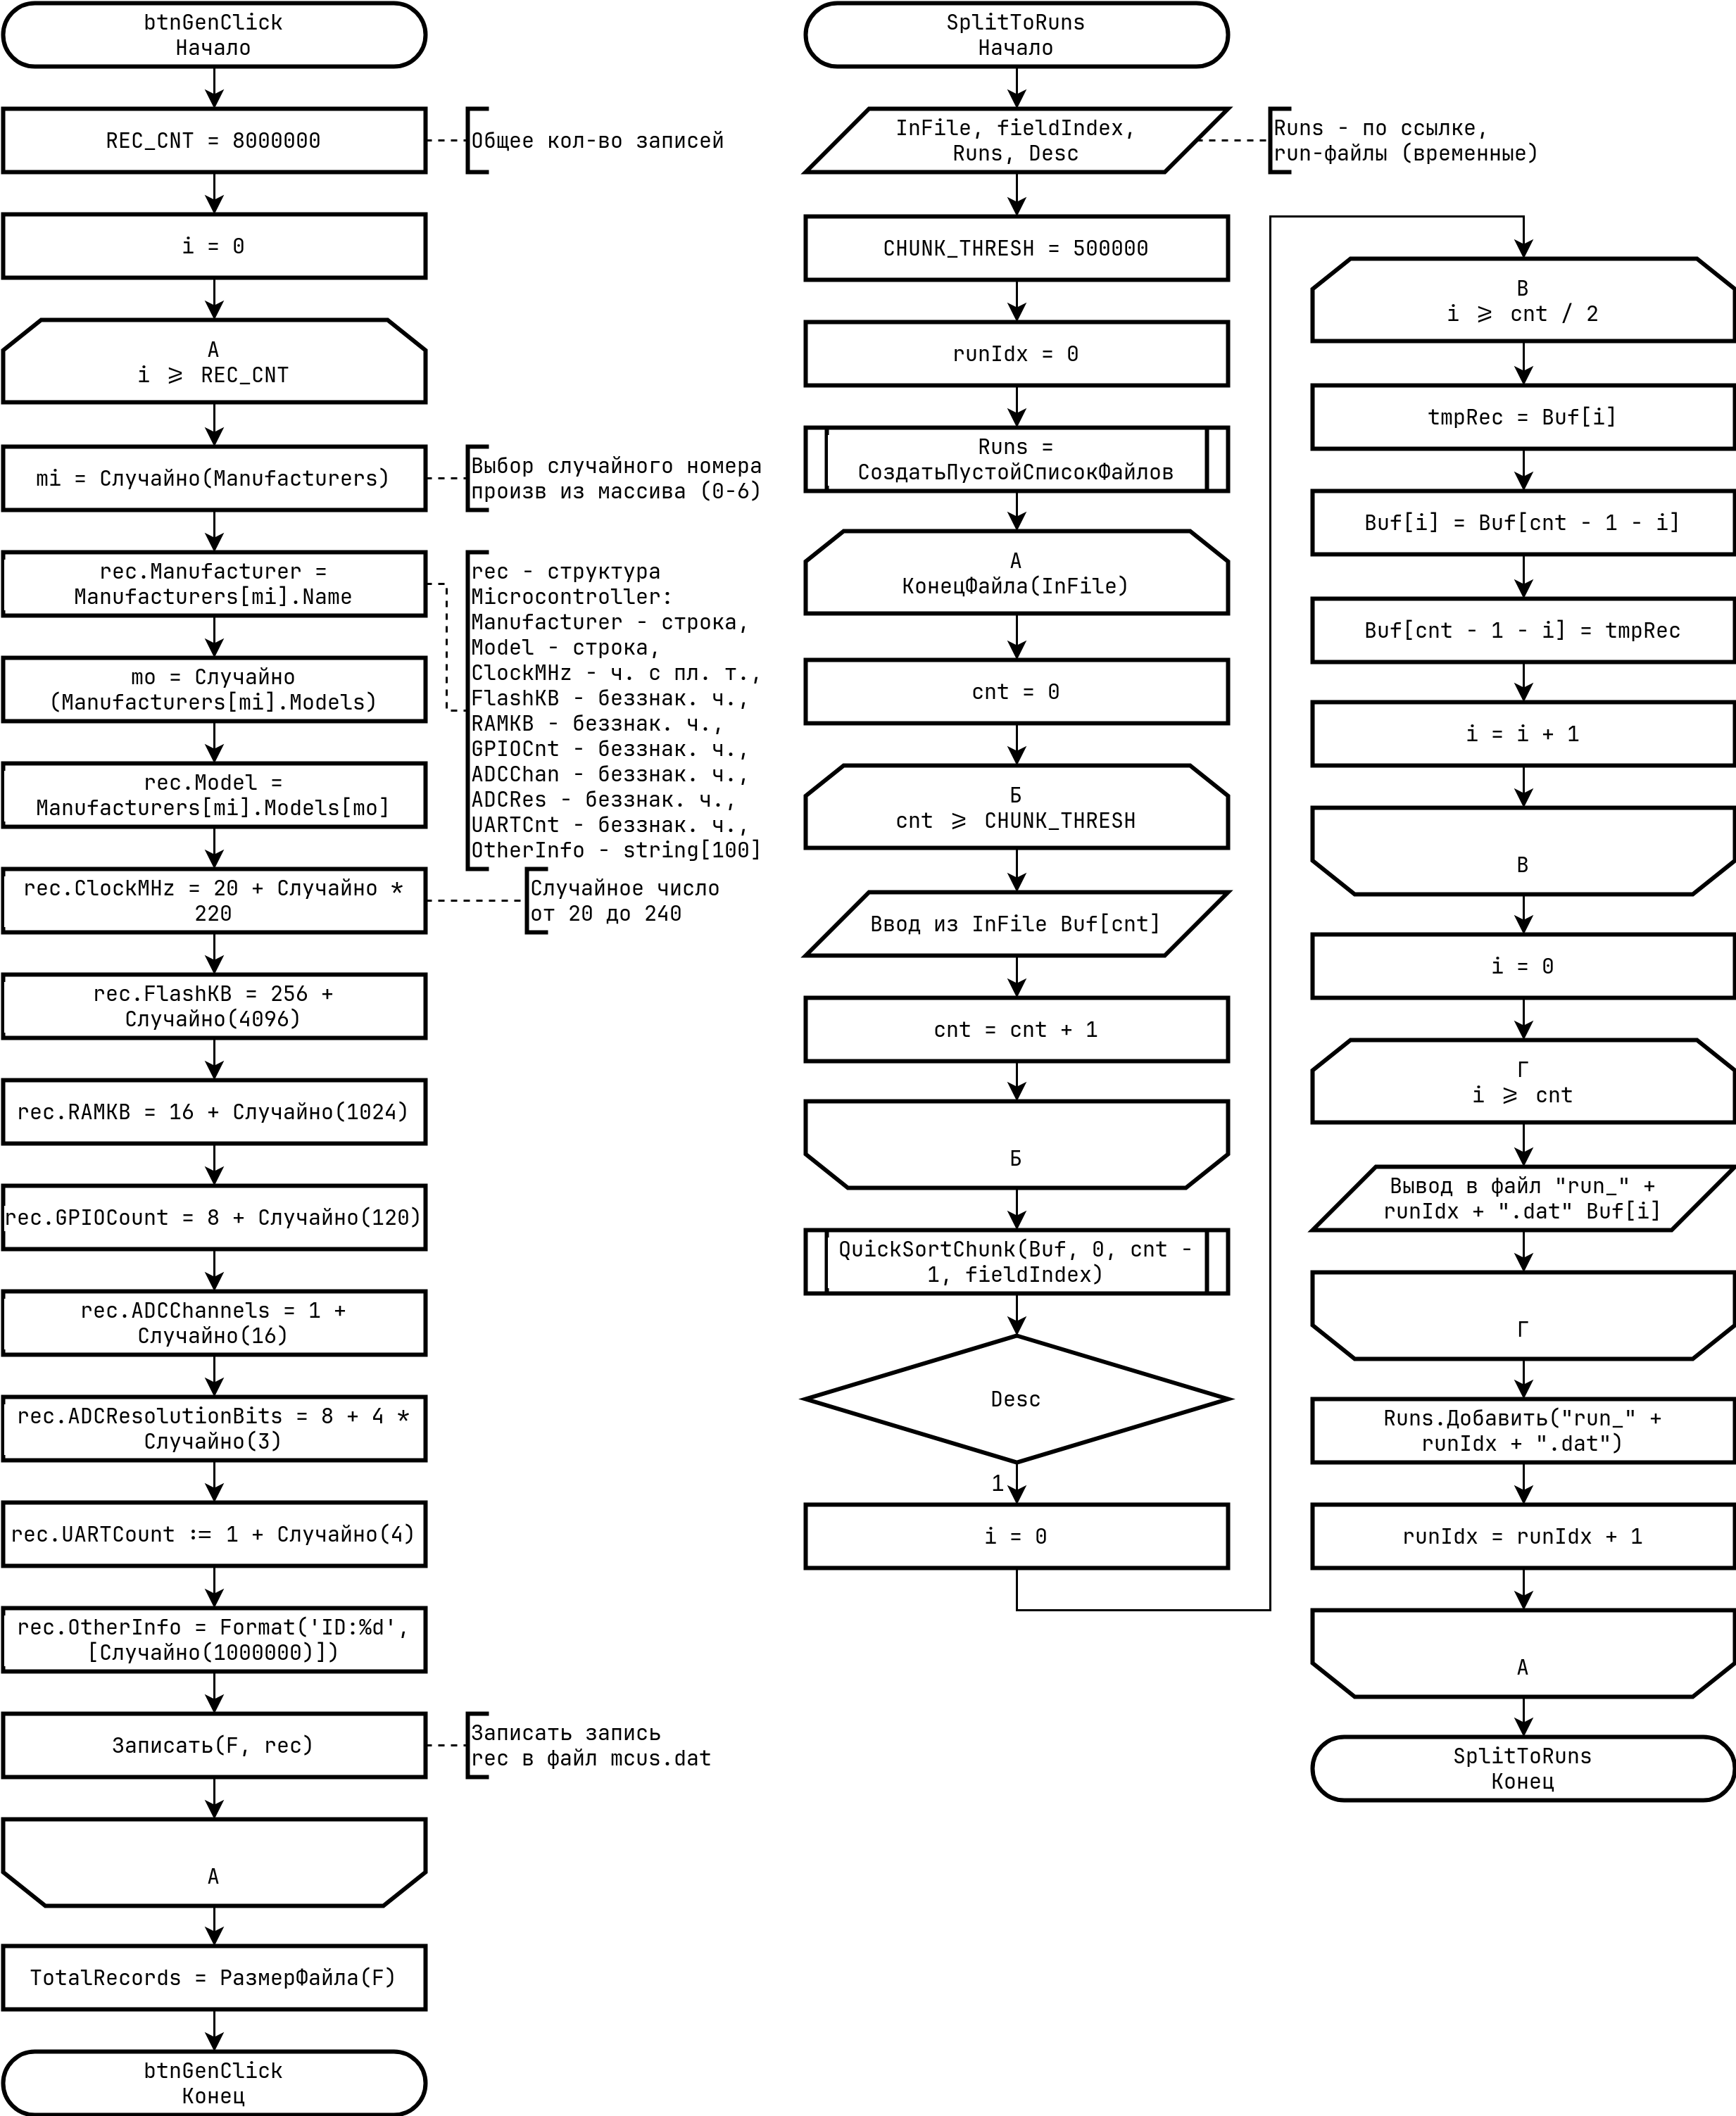
\includegraphics[height=0.9\textheight]{pics/flowchart3.png}
	\caption*{Рисунок 1.3 - Схемы алгоритмов подпрограмм нажатия на кнопку Генерация, разбиения на временные(ран-файлы).}
\end{figure}

\clearpage
\begin{figure}[H]
	\centering
	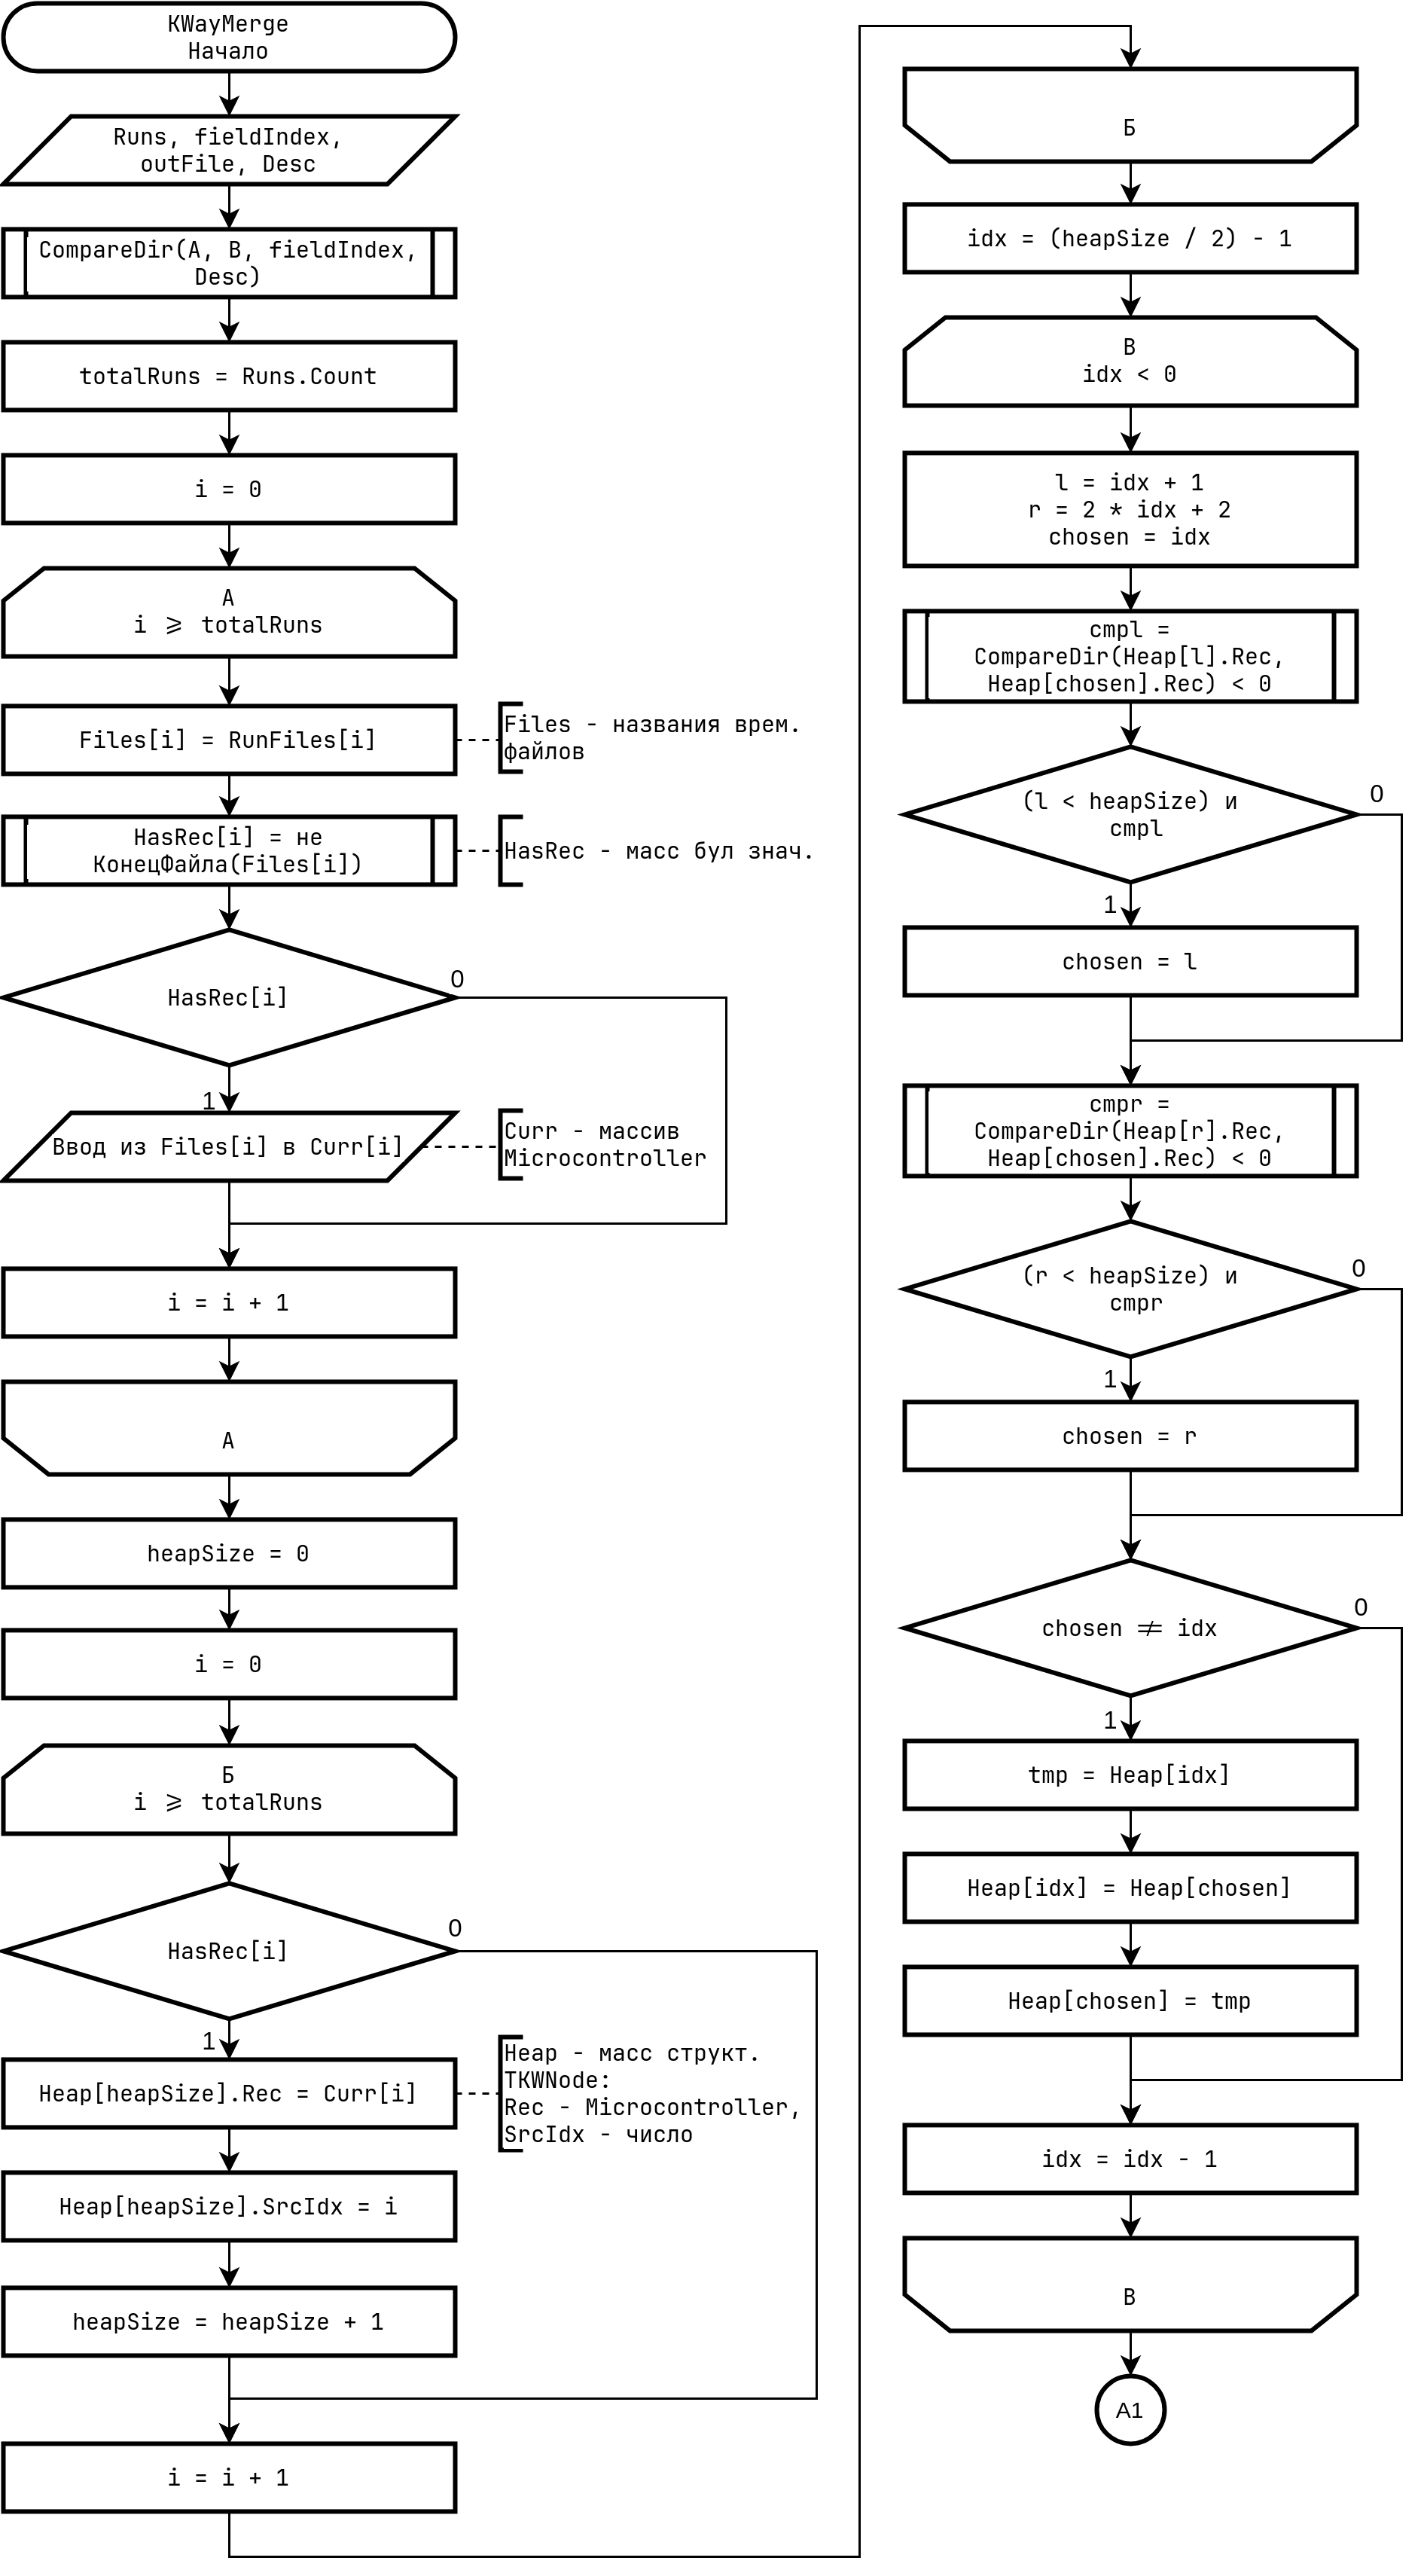
\includegraphics[height=0.9\textheight]{pics/flowchart4p1.png}
	\caption*{Рисунок 1.4.1 - Схема алгоритма подпрограммы многопутевого слияния ч.1.}
\end{figure}

\clearpage
\begin{figure}[H]
	\centering
	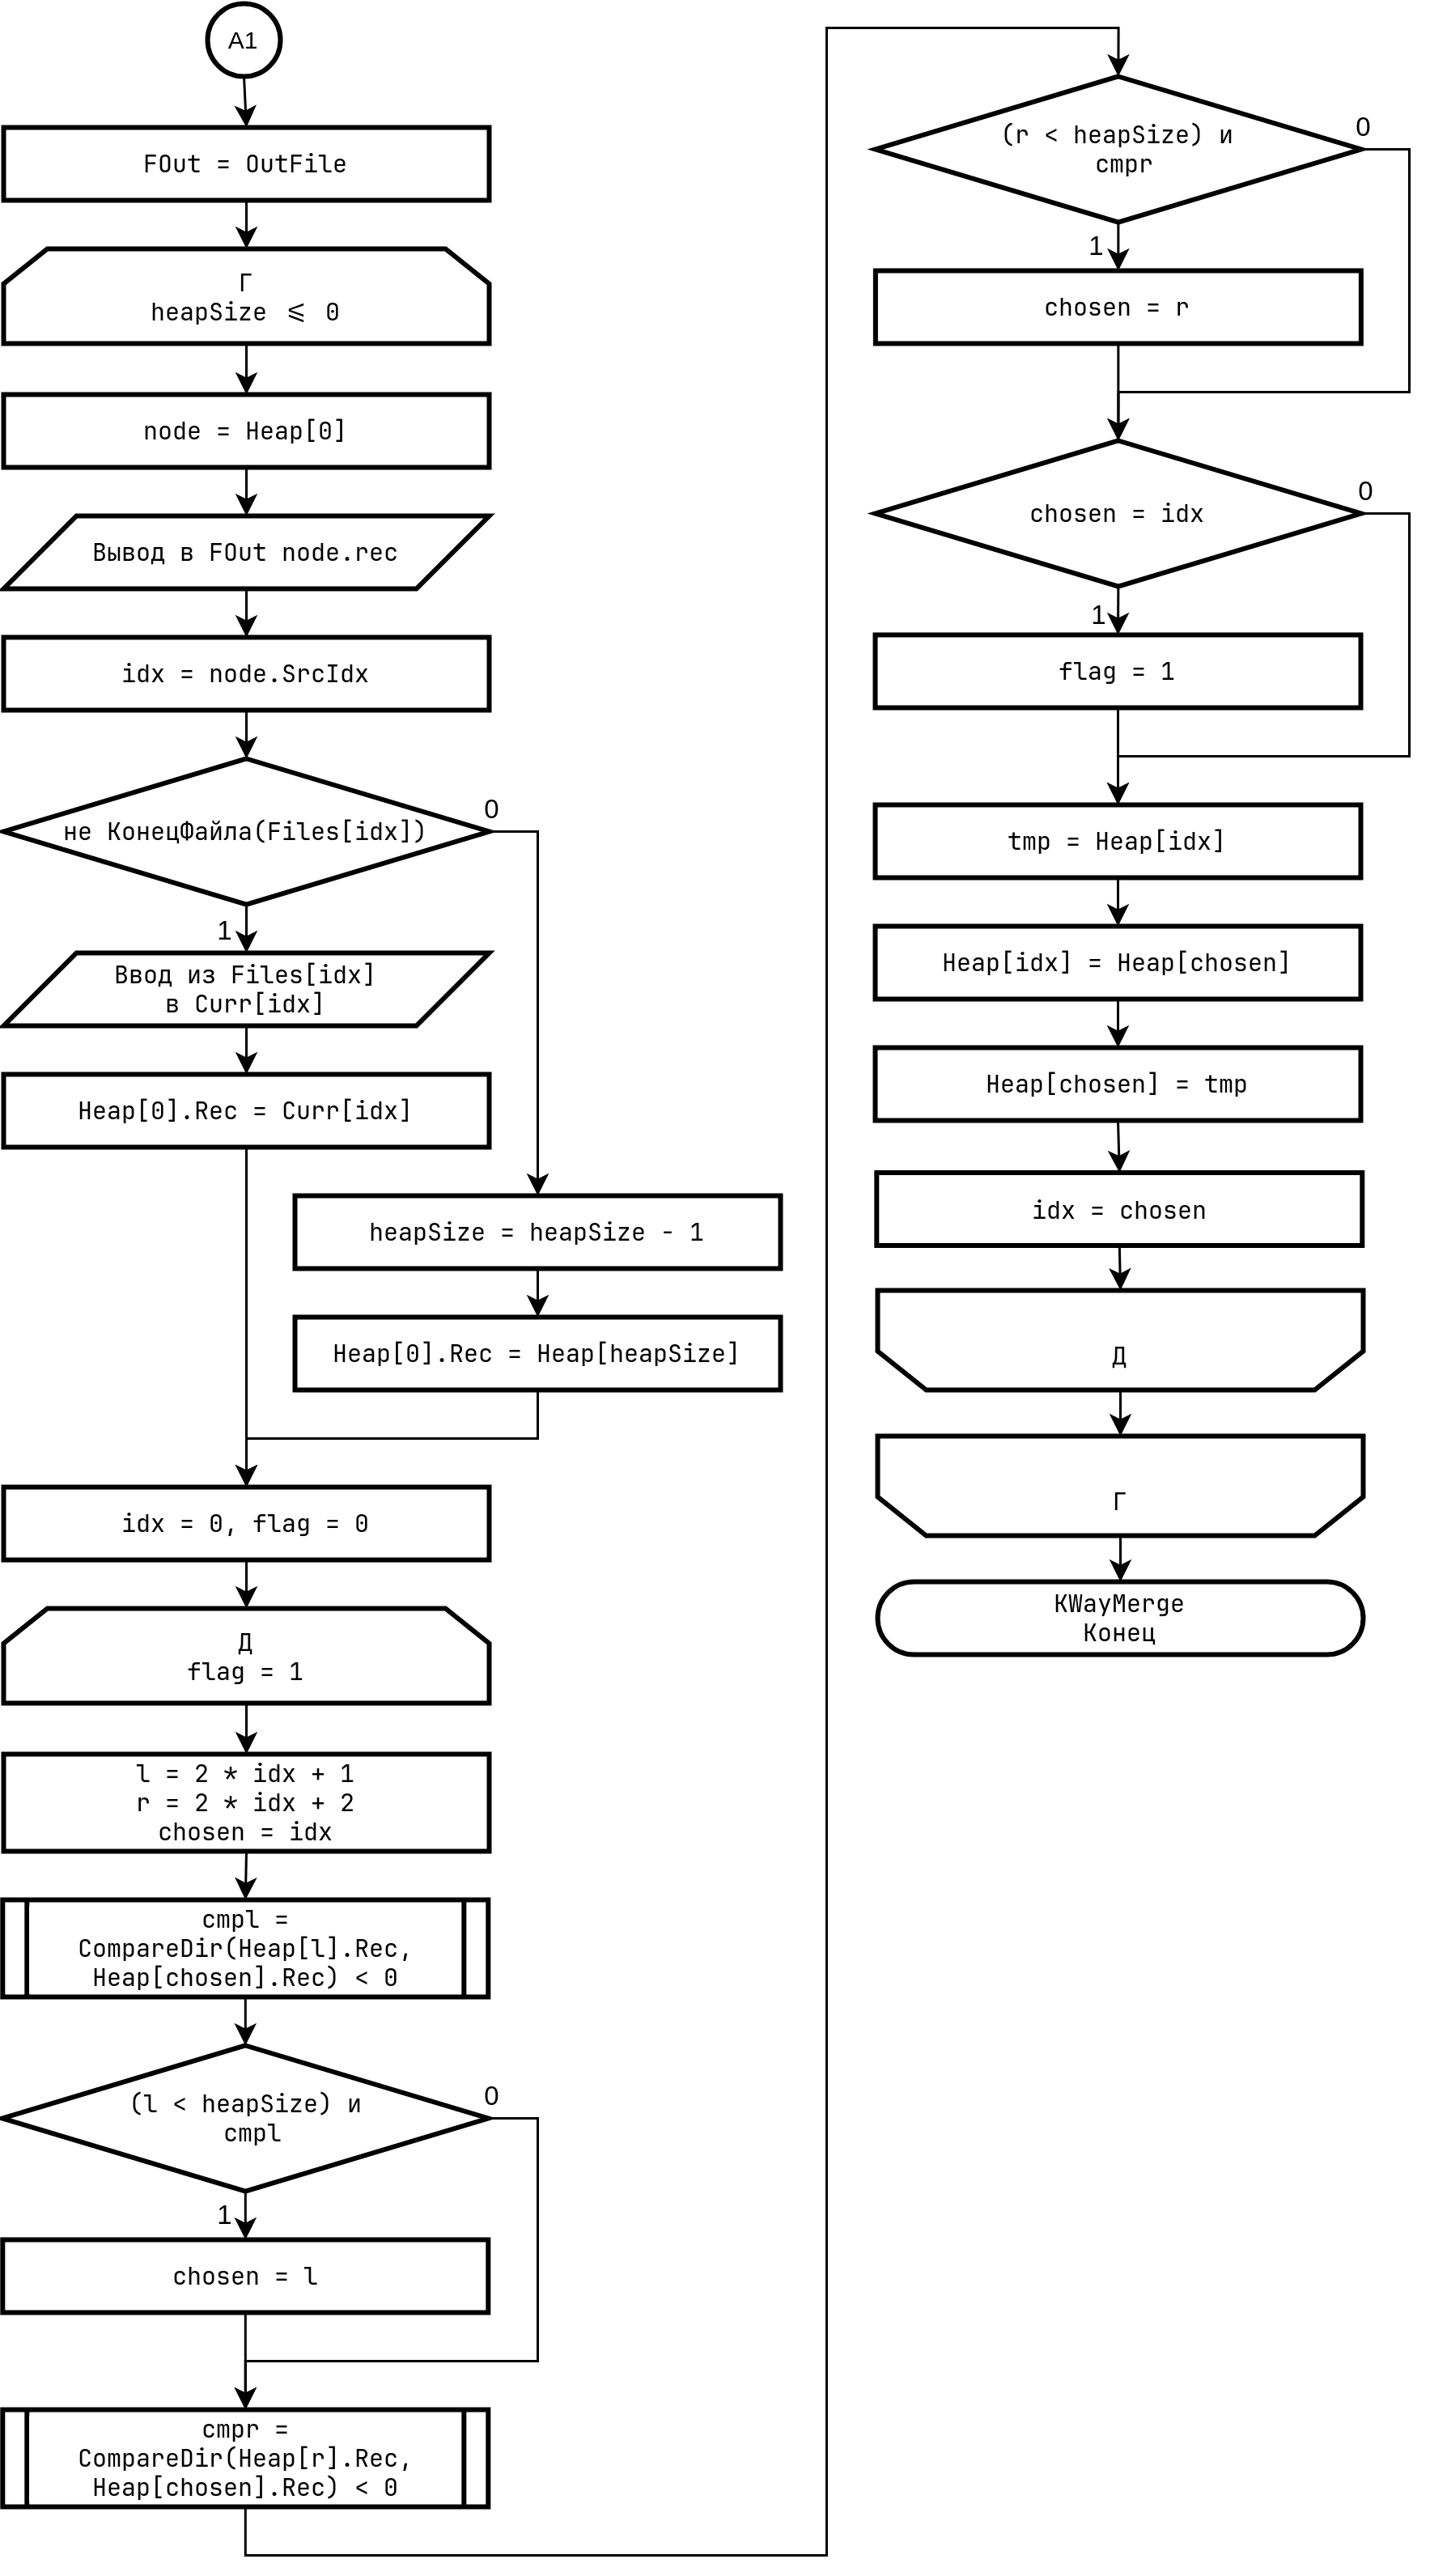
\includegraphics[height=0.9\textheight]{pics/flowchart4p2.png}
	\caption*{Рисунок 1.4.2 - Схема алгоритма подпрограммы многопутевого слияния ч.2.}
\end{figure}

\clearpage
\begin{figure}[H]
	\centering
	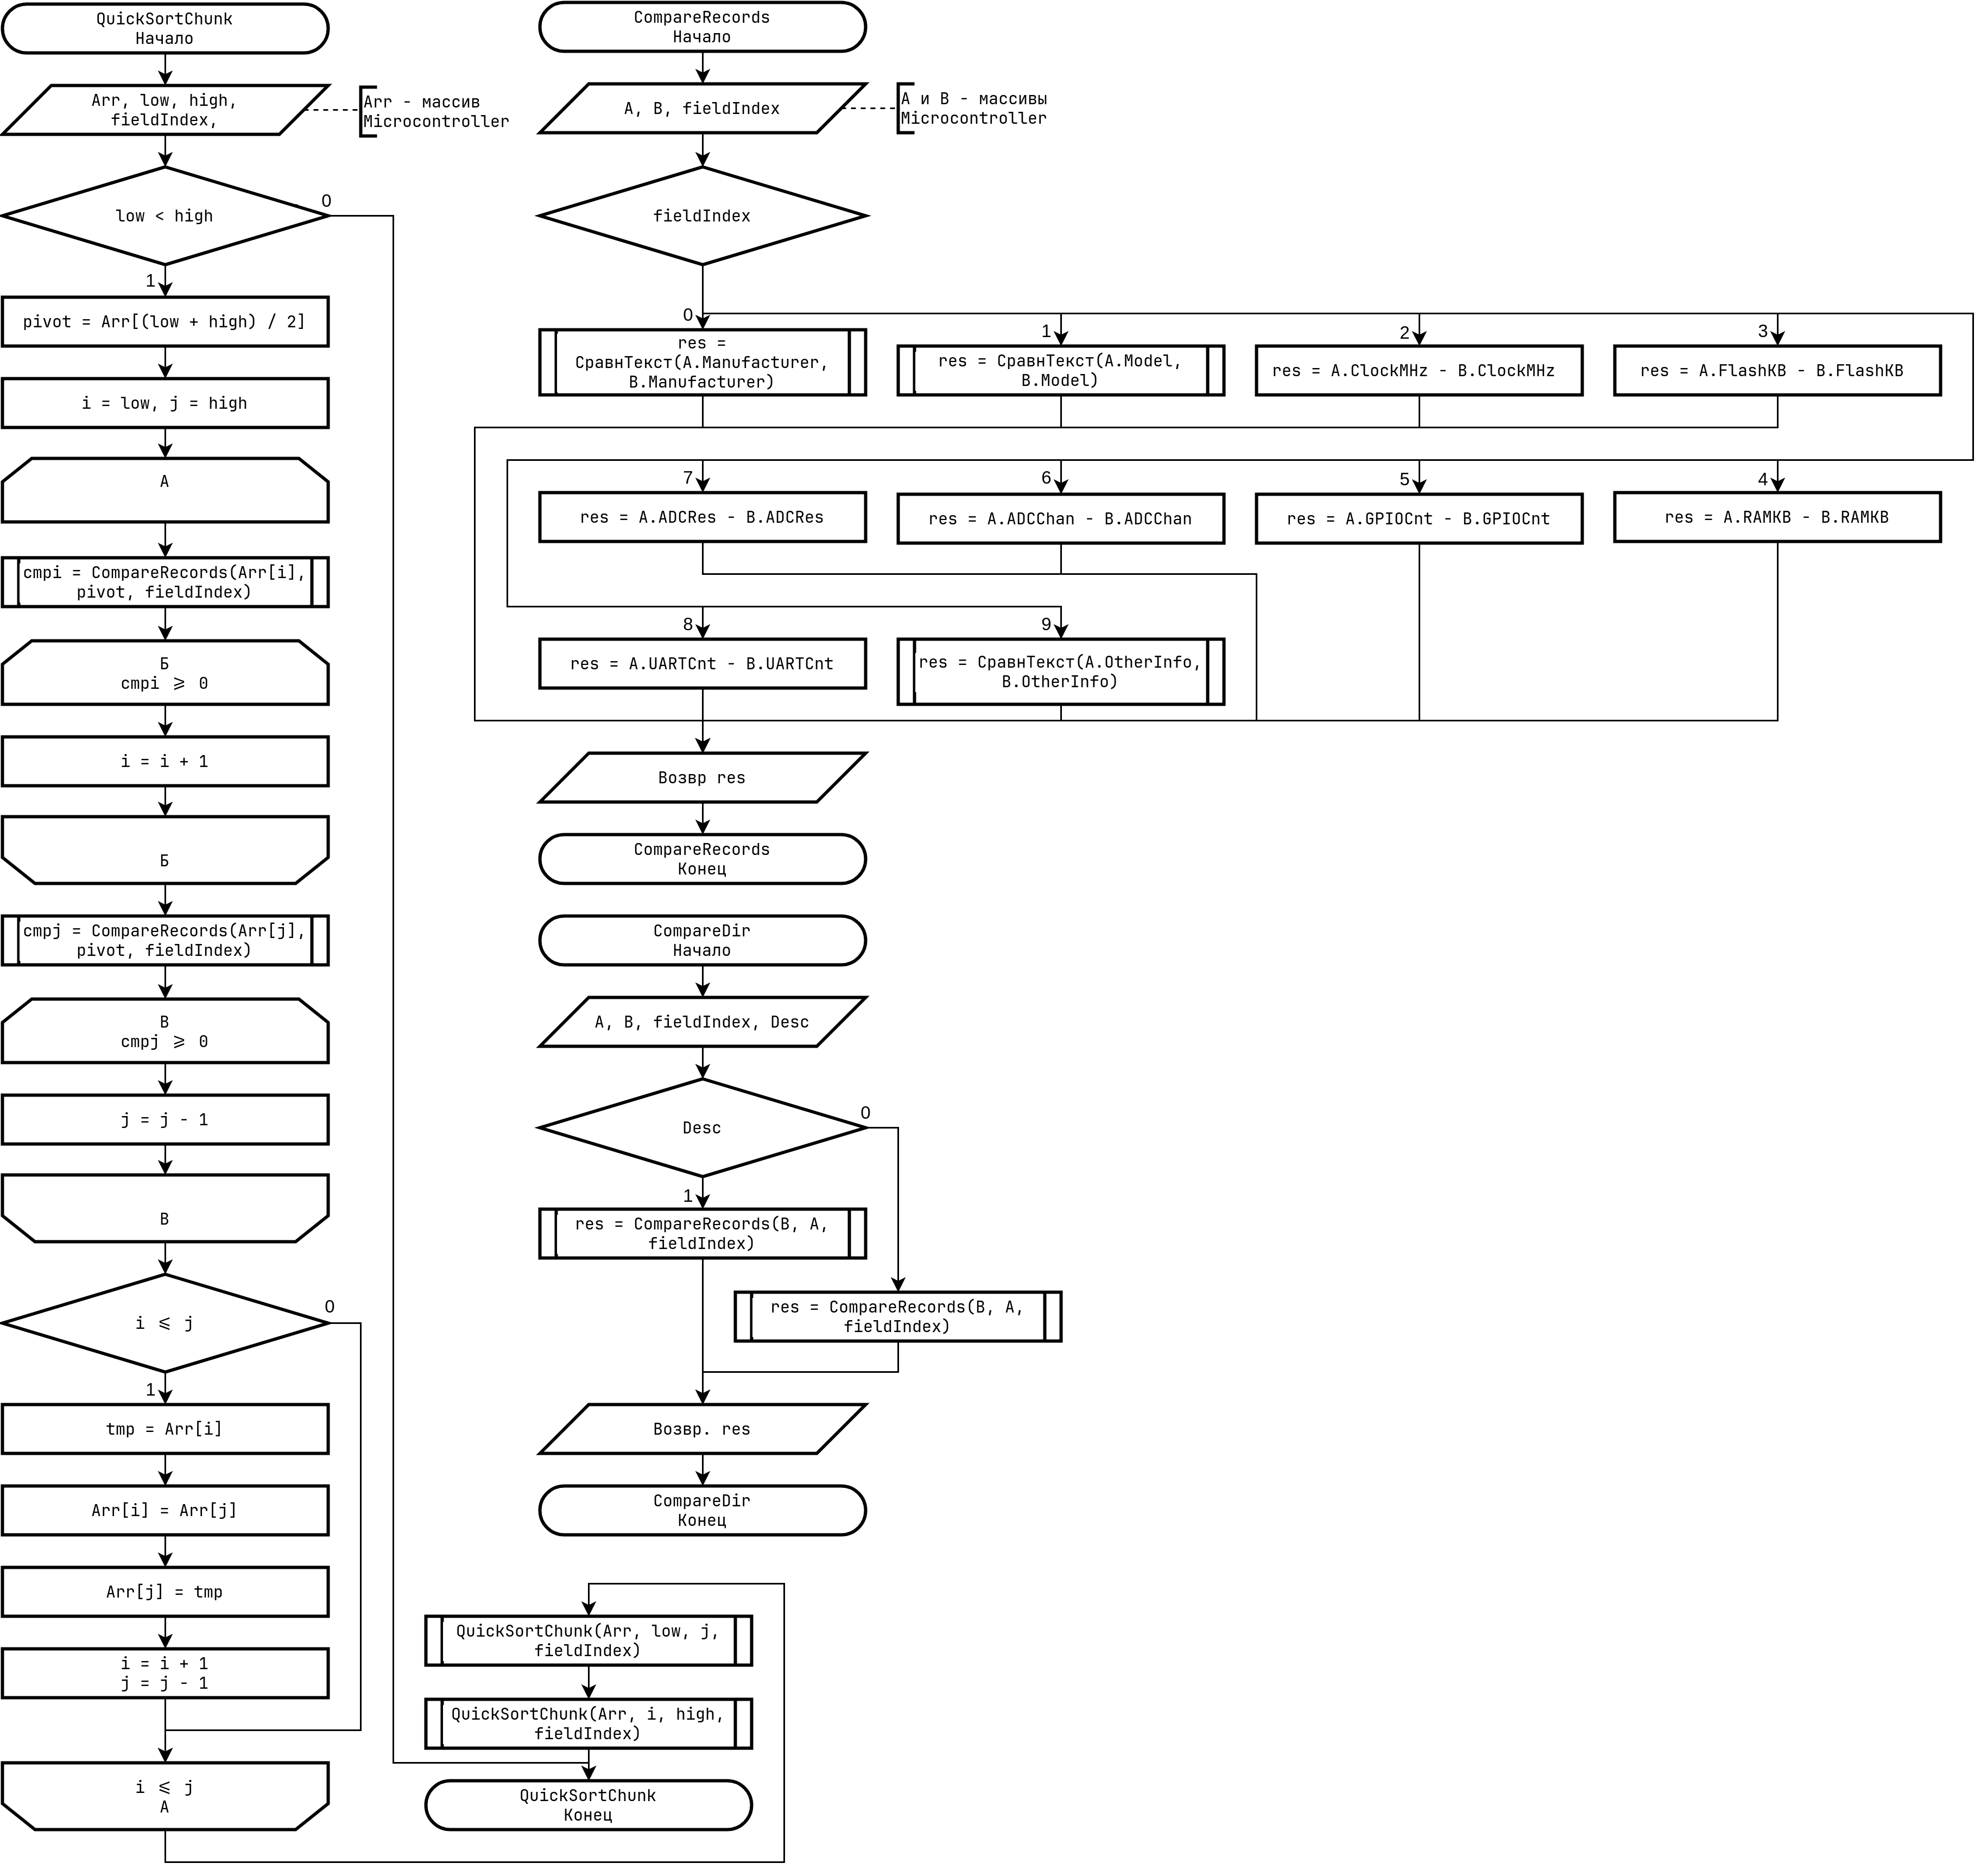
\includegraphics[width=0.9\textwidth]{pics/flowchart5.png}
	\caption*{Рисунок 1.5 - Схема алгоритма подпрограммы быстрой сортировки чанка и подпрограммы сравнения двух элементов из списка по полю.}
\end{figure}

\clearpage
\begin{figure}[H]
	\centering
	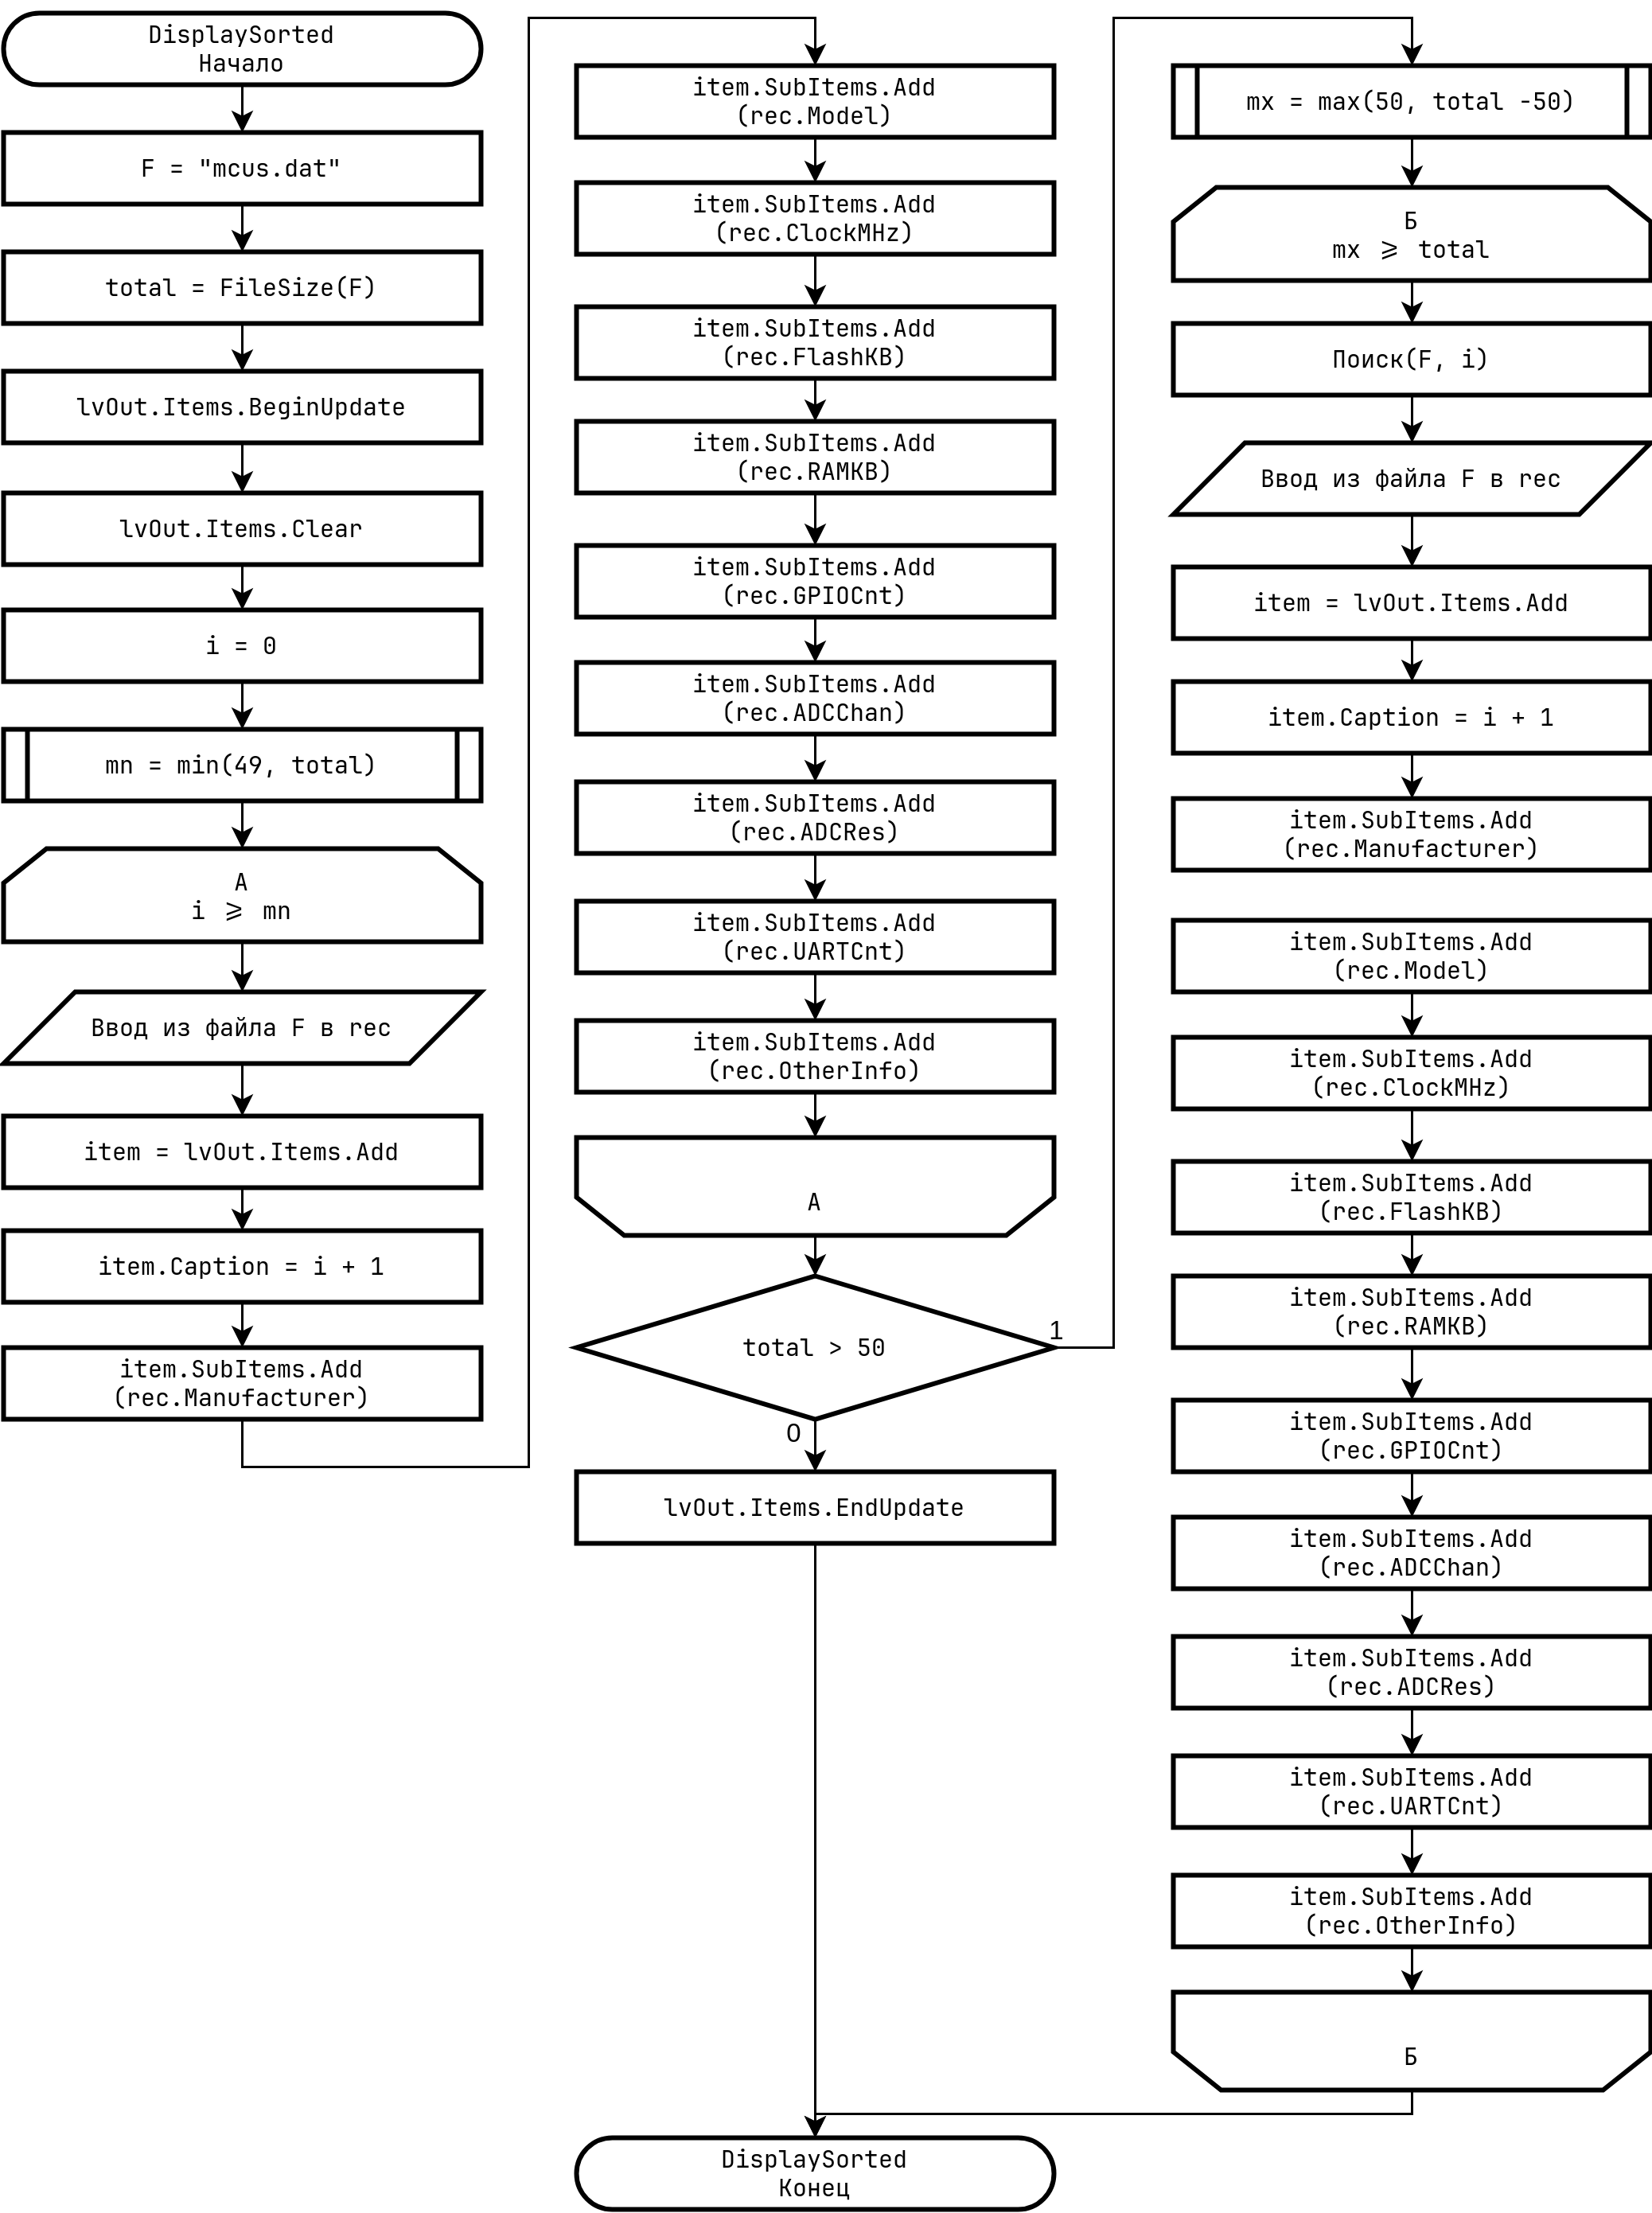
\includegraphics[height=0.9\textheight]{pics/flowchart6.png}
	\caption*{Рисунок 1.6 - Схема алгоритма подпрограммы вывода отсортированного списка.}
\end{figure}

\section*{Вывод}

В ходе лабораторной работы была разработана программа с графическим интерфейсом для внешней сортировки файлов, что позволило освоить алгоритмы многопутевого слияния и работу с файлами в Lazarus.

\newpage

\setminted{style = rainbow_dash, fontsize = \small} % https://pygments.org/styles/

\section*{Приложение А1. Исходный код}
\inputminted{pas}{code/lab8_unit.pas}

\end{document}
